\section{Computing with Turing Machines}
\label{sec:compute-w-tm}

We adopt the following policy for presenting input to Turing machines: 
\begin{itemize}
  \item The input string which has \textit{no blank symbols in it}, is written to the right of the leftmost symbol $\tar$, with a \textit{blank to its left}, and \textit{blanks to its right}; 
  \item The head is positioned at the tape square containing the blank between the $\tar$ and the input; 
  \item The machine starts operating in its initial state.
\end{itemize}
If $M = (K, \Sigma, \delta, s, H)$ is a Turing machine and $w \in (\Sigma - \{ \blank, \tar \})^*$, then the \textbf{initial configuration of $M$ on input} $w$ is $(s, {\tar}{\underline{\blank}}w)$. With this convention, we can now define how Turing machines are used as language recognizers.

\begin{definition}{}
\quad Let $M = (K, \Sigma, \delta, s, H)$ be a Turing machine, such that $H = \{ y, n \}$ consists of two distinguished halting states ($y$ and $n$ for ``yes'' and ``no''). Any halting configuration whose state component is $y$ is called an \textbf{accepting configuration}, while a halting configuration whose state component is $n$ is called a \textbf{rejecting configuration}. \\

We say that $M$ \textbf{accepts} an input $w \in (\Sigma - \{ \blank, \tar \})^*$ if $(s, {\tar}{\underline{\blank}}w)$ yields an accepting configuration; we say that $M$ \textbf{rejects} $w$ if $(s, {\tar}{\underline{\blank}}w)$ yields a rejecting configuration. \\

\quad Let $\Sigma_0 \subseteq \Sigma - \{ \blank, \tar \}$ be an alphabet, called the \textbf{input alphabet} of $M$; by fixing $\Sigma_0$ to be a subset of $\Sigma - \{ \blank, \tar \}$, we allow our Turing machines to use extra symbols during their computation, besides those appearing in their inputs. We say that $M$ \textbf{decides} a language $L \subseteq \Sigma_0^*$ if for any string $w \in \Sigma_0^*$ the following is true: ``If $w \in L$ then $M$ accepts $w$; and if $w \notin L$ then $M$ rejects $w$''. \\

\quad Finally, call a language $L$ \textbf{recursive} if there is a Turing machine that decides it.
\end{definition}
That is, a Turing machine decides a language $L$ if, when started with input $w$, it always halts, and does so in a halt state that is the correct response to the input: $y$ if $w \in L$, $n$ if $w \notin L$. Notice that no guarantees are given about what happens if the input to the machine contains blanks or the left end symbol.

\begin{figure}[H]
  \centering
  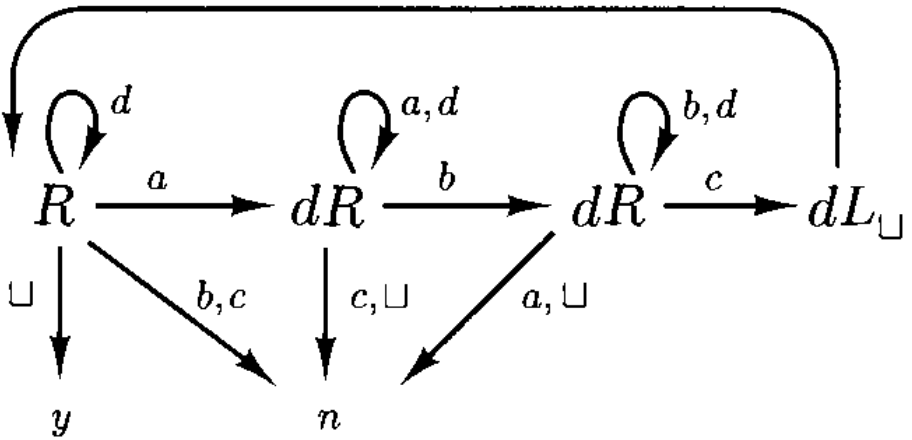
\includegraphics[width=\linewidth]{img/fig-4.11.png}
  \caption{}
  \label{fig:4.7}
\end{figure}

\begin{example}{}
\quad Consider the language $L = \{ a^nb^nc^n\ |\ n \geq 0 \}$, which has heretofore evaded all types of language recognizers. The Turing machine whose diagram is shown in Figure 7 decides $L$. In this diagram we have also utilized two new basic machines, useful for deciding languages: Machine $y$ makes the new state to be the accepting state $y$, while machine $n$ moves the state to $n$. \\

\quad The strategy employed by $M$ is simple: On input $a^nb^nc^n$ it will operate in $n$ stages. In each stage $M$ starts from the left end of the string and moves to the right in search of an $a$. 
\begin{itemize}
  \item When it finds an $a$, it replaces it by a $d$ and then looks further to the right for a $b$.
  \item When a $b$ is found, it is replaced by a $d$, and the machine then looks for a $c$.
  \item When a $c$ is found and is replaced by a $d$, then the stage is over, and the head returns to the left end of the input. Then the next stage begins. \newline
\end{itemize}

\quad That is, at each stage the machine replaces an $a$, a $b$, and a 
$c$ by $d$'s. If at any point the machine senses that the string is not in $a^*b^*c^*$, or that there is an excess of a certain symbol (for example, if it sees a $b$ or $c$ while looking for an $a$), then it enters state $n$ and rejects immediately. \\

\quad If however it encounters the right end of the input while looking for an $a$, this means that all the input has been replaced by $d$'s, and hence it was indeed of the form $a^nb^nc^n$, for some $n \geq 0$. The machine then accepts.
\end{example}

There is a subtle point in relation to Turing machines that decide languages: With the other language recognizers that we have seen so far (even the nondeterministic ones), one of two things could happen: Either
\begin{itemize}
  \item the machine accepts the input, or 
  \item the machine rejects the input.
\end{itemize}
A Turing machine, on the other hand, even if it has only two halt states $y$ and $n$, always has the option of evading an answer (``yes'' or ``no''), by failing to halt. Given a Turing machine, it might or it might not decide a language (and there is no obvious way to tell whether it does). The far-reaching importance (and necessity) of this deficiency will become apparent later in this chapter, and in the next.

\vspace*{\fill}
\columnbreak

\subsection{Recursive Functions}

Since Turing machines can write on their tapes, they can provide more elaborate output than just a ``yes'' or a ``no'':
\begin{definition}{}
Let $M = (K, \Sigma, \delta, s, \{h\})$ be a Turing machine, let $\Sigma_0 \subseteq \Sigma - \{ \blank, \tar \}$ be an alphabet, and let $w \in \Sigma_0^*$. Suppose that $M$ halts on input $w$, and that $(s,\ {\tar}{\underline{\blank}}w) \vdash_M^* (h,\ {\tar}{\underline{\blank}}y)$ for some $y \in \Sigma_0^*$. Then $y$ is called the \textbf{output} of $M$ on input $w$, and is denoted $M(w)$. Notice that $M(w)$ is defined \textit{only if $M$ halts on input $w$}, and in fact does so at a configuration of the form $(h,\ {\tar}{\underline{\blank}}y)$ with $y \in \Sigma_0^*$. \\

\quad Now let $f$ be any function from $\Sigma_0^*$ to $\Sigma_0^*$. We say that $M$ \textbf{computes} function $f$ if, for all $w \in \Sigma_0^*$, $M(w) = f(w)$. That is, for all $w \in \Sigma_0^*$, $M$ eventually halts on input $w$, and when it does halt, its tape contains the string ${\tar}{\underline{\blank}}f(w)$. A function $f$ is called \textbf{recursive}, if there is a Turing machine $M$ that computes $f$. 
\end{definition}

\begin{example}{}
The function $\kappa: \Sigma^* \mapsto \Sigma^*$ defined as $\kappa(w) = ww$ can be computed by the machine $CS_{\la}$, that is, the copying machine followed by the left-shifting machine.
\end{example}

Strings in $\{ 0, 1 \}^*$ can be used to represent the nonnegative integers in the familiar \textit{binary notation}. Any string $w = a_1a_2 \ldots a_n \in \{ 0, 1 \}^*$ represents the number 
\begin{equation*}
  num(w) = a_1 \cdot 2^{n-1} + a_2 \cdot 2^{n-2} + \ldots + a_n.
\end{equation*}
And any natural number can be represented in a unique way by a string in $0 \cup 1(0 \cup 1)^*$ (that is to say, without redundant 0's in the beginning).

Accordingly, Turing machines computing functions from $\{ 0, 1 \}^*$ to $\{ 0, 1 \}^*$ can be thought of as computing functions from the natural numbers to the natural numbers. In fact, numerical functions with many arguments (such as addition and multiplication) can be computed by Turing machines computing functions from $\{ 0, 1, ; \}^*$ to $\{ 0, 1 \}^*$, where ``$;$'' is a symbol used to separate binary arguments. 

\begin{definition}{}
Let $M = (K, \Sigma, \delta, s, \{h\})$ be a Turing machine such that $0, 1, ; \in \Sigma$, and let $f$ be any function from $\mathbf{N^k}$ to $\mathbf{N}$ for some $k \geq 1$. We say that $M$ \textbf{computes} function $f$ if for all $w_1, \ldots, w_k \in 0 \cup 1(0 \cup 1)^*$ (that is, for any $k$ strings that are binary encodings of integers), $\texttt{num}(M(w_1; \ldots; w_k)) = f(num(w_1), ... ,num(w_k))$. \\

\quad That is, if $M$ is started with the binary representations of the integers $n_1, ..., n_k$ as input, then it eventually halts, and when it does halt, its tape contains a string that represents number $f(n_1, ..., n_k)$ -the value of the function. A function $f\ :\ N^k \mapsto N$ is called \textbf{recursive} if there is a Turing machine $M$ that computes $f$.
\end{definition}

On our inability to tell whether a Turing machine decides a language, also applies to function computation. The price we must pay for the very broad range of functions that Turing machines can compute, is that we cannot tell whether a given Turing machine indeed computes such a function -that is to say, whether it halts on all inputs.

\subsection{Recursively Enumerable Languages}

If a Turing machine decides a language or computes a function, it can be reasonably thought of as an algorithm that performs correctly and reliably some computational task. We next introduce a third, subtler, way in which a Turing machine can define a language: 
\begin{definition}{}
Let $M = (K, \Sigma, \delta, s, H)$ be a Turing machine, let $\Sigma_0 \subseteq \Sigma - \{ \blank, \tar \}$ be an alphabet, and let $L \subseteq \Sigma_0^*$ be a language. We say that $M$ \textbf{semidecides} $L$ if for any string $w \in \Sigma_0^*$ the following is true:
\begin{quote}
  $w \in L$ if and only if $M$ halts on input $w$.
\end{quote}
A language $L$ is \textbf{recursively enumerable} if and only if there is a Turing machine $M$ that semidecides $L$.
\end{definition}

Thus when $M$ is presented with input $w \in L$, it is required to halt eventually. We \textit{do not care precisely which halting configuration it reaches}, as long as it does eventually arrive at a halting configuration. If however $w \in \Sigma_0^* - L$, then $M$ must never enter the halting state; that is, the machine must continue its computation indefinitely.

Extending the ``functional'' notation of Turing machines that we introduced in the previous subsection (which allows us to write equations such as $M(w) = v$), we shall write $M(w) = \nearrow$ if $M$ fails to halt on input $w$. In this notation, we can restate the definition of semidecision of a language $L \subseteq \Sigma_0^*$ by Turing machine $M$ as follows:
\begin{quote}
  For all $w \in \Sigma_0^*$, $M(w) = \nearrow$ if and only if $w \notin L$.
\end{quote}

\begin{example}{}

Let $L = \{ w \in \{a, b\}^*\ |\ w \textnormal{ contains at least one } a \}$. Then $L$ is semidecided by the Turing machine shown in Figure 8.
\begin{figure}[H]
  \centering
  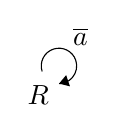
\begin{tikzpicture}[scale=0.15]
    \tikzstyle{every node}+=[inner sep=0pt]
    \draw (0.9,-5.6) node {$R$};
    \draw [black] (1.227,-3.635) arc (198.28227:-89.71773:1.5);
    \draw (4.47,-1.45) node [above] {$\overline{a}$};
    \fill [black] (2.66,-4.66) -- (3.58,-4.89) -- (3.26,-3.94);
  \end{tikzpicture}
  \caption{}
  \label{fig:4.8}
\end{figure}
\quad This machine, when started in configuration $(q_0,\ {\tar}{\underline{\blank}}w)$ for some $w \in \{ a, b \}^*$, simply scans right until an $a$ is encountered and then halts. If no $a$ is found, the machine goes on forever into the blanks that follow its input, never halting.

\quad So $L$ is exactly the set of strings $w$ in $\{ a, b \}^*$ such that $M$ halts on input $w$. Therefore $M$ semidecides $L$, and thus $L$ is recursively enumerable.
\end{example}

The definition of semidecision by Turing machines is a rather straightforward extension of the notion of acceptance for the deterministic finite automaton. There is a major difference, however. A finite automaton always halts when it has read all of its input -the question is whether it halts on a final or a non final state. In this sense it is a useful computational device, an \textit{algorithm} from which we can reliably obtain answers as to whether an input belongs in the accepted language: We wait until all of the input has been read, and we then observe the state of the machine.

In contrast, a Turing machine that semidecides a language $L$ cannot be usefully employed for telling whether a string $w$ is in $L$, because, if $w \notin L$, then \textit{we will never know when we have waited enough for an answer}. Turing machines that semidecide languages are no algorithms.

$\{ a^nb^nc^n\ |\ n \geq 0 \}$ is a recursive language. But is it recursively enumerable? $\{ a^nb^nc^n\ |\ n \geq 0 \}$ is also recursively enumerable. Actually, \textit{Any recursive language is also 1'ecursively enumerable} as stated in theorem 2.1. All it takes in order to construct another Turing machine that semidecides, instead of decides, the language is to make the rejecting state $n$ a nonhalting state, from which the machine is guaranteed to never halt.

Specifically, given any Turing machine $M = (K, \Sigma, \delta, s, \{y, n\})$ that decides $L$, we can define a machine $M'$ that semidecides $L$ as follows: $M = (K, \Sigma, \sigma', s, \{y\})$, where $\delta'$ is just $\delta$ augmented by the following transitions related to $n$ -no longer 
a halting state: $\delta'(n, a) = (n, a)$ for all $a \in \Sigma$.

It is clear that if $M$ indeed decides $L$, then $M'$ semidecides $L$, because $M'$ accepts the same inputs as $M$; furthermore, if $M$ rejects an input $w$, then $M'$ does not halt on $w$ (it ``loops forever'' in state $n$). In other words, for all inputs $w$, $M'(w) = \nearrow$ if and only if $M(w) = n$.

\begin{theorem}{}
  If a language is recursive, then it is recursively enumerable.
\end{theorem}

Naturally, the interesting (and difficult) question is the opposite:
\begin{quote}
  Can we always transform every Turing machine that semidecides a language into an actual algorithm for deciding the same language?
\end{quote}
We shall see in the next chapter that the answer here is negative: 
\begin{quote}
  There are recursively enumerable languages that are not recursive.
\end{quote}

An important property of the class of recursive languages is that it is closed under complement: 
\begin{theorem}{}
  If $L$ is a recursive language, then its complement $\overline{L}$ is also recursive.
\end{theorem}

\vspace*{\fill}
\columnbreak

\begin{proof}
  If $L$ is decided by Turing machine $M = (K, \Sigma, \delta, s, \{y, n\})$, then $L$ is decided by the Turing machine $M' = (K, \Sigma, \delta', s, \{y, n\})$ which is identical to $M$ \textit{except that it reverses the roles of the two special halting states $y$ and $n$}. That is, $\delta'$ is defined as follows:
  \begin{equation*}
    \delta'(q, a) = 
      \begin{cases}
        n             &\textnormal{if } \delta(q, a) = y \\
        y             &\textnormal{if } \delta(q, a) = n \\
        \delta(q, a)  &\textnormal{otherwise}
      \end{cases}
  \end{equation*}
  It is clear that $M'(w) = y$ if and only if $M(w) = n$, and therefore $M'$ decides $\overline{L}$.
\end{proof}
